\documentclass[a4paper, 10pt]{article}
\usepackage[utf8]{inputenc}
\usepackage[spanish]{babel}
\usepackage{graphicx}
\usepackage{geometry}
\usepackage{listings}
\usepackage{amsmath}
\usepackage{amsfonts}
\usepackage{amssymb}
\usepackage{caratula}

\newcommand{\Z}{\mathbb{Z}}
\def\code#1{\texttt{#1}}
\newcommand\tab[1][0.5cm]{\hspace*{#1}}

\geometry{a4paper, margin=0.7in}

\begin{document}
    %Caratula
    \pagenumbering{gobble}
    \newpage

    \begin{center}
        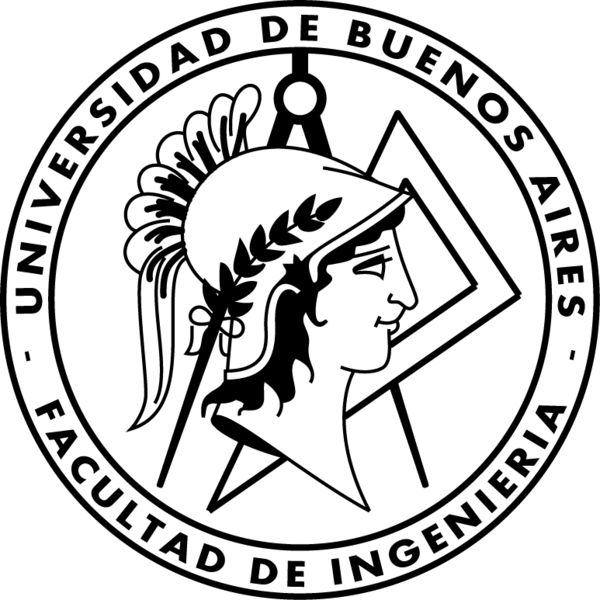
\includegraphics{images/logo}
    \end{center}

    \materia{Teoría de Algoritmos 2}
    \submateria{Segundo Cuatrimestre 2017}
    \titulo{Trabajo Práctico 1}

    \integrante{Rodrigo De Rosa}{97799}{rodrigoderosa@outlook.com}
    \integrante{Marcos Schapira}{97934}{schapiramarcos@gmail.com}
    \integrante{Facundo Guerrero}{97981}{facundoiguerrero@gmail.com}
    \maketitle
    %Fin caratula
    %Table of contents
    \newpage
    \pagenumbering{roman}
    \tableofcontents
    %Fin table of contents
    %Informe
    \newpage
	\pagenumbering{arabic}
	
	\section{Rabin - Karp}
		
		\emph{Algoritmo Michael O. Rabin and Richard M. Karp 1987}
		
		\subsection{Funcionamiento}
		\tab La idea del algoritmo es muy simple. Basándose en la estructura del algoritmo naïve, este 				agrega un paso previo que compara los strings por valores de hash. Para esto precisa una función de 		hash que se busca que compare entre valores lo mas rápido posible. Esto tiene el potencial 					beneficio de acortar los tiempos de comparación entre strings mientras que agrega la complejidad 			del calculo previo del valor de hash para cada string.
		
		\subsection{Implementación}
		
		La implementación es muy simple. Primero calcula el valor de hash para el patrón a buscar. Luego recorre el texto calculando el valor de hash para la palabra a buscar. Compara ambos valores y si dan iguales entonces compara si las palabras son realmente iguales o no. Para ganar mayor velocidad se utilizo la librería pyhash \footnote{https://github.com/flier/pyfasthash} que contiene implementaciones en C/C++ para mejor eficiencia de algoritmos no criptográficos. De estos se usaron (todos de 32 bits): FNV, Murmur Hash, City Hash, Spooky Hash.
		
		\subsection{Complejidad}
		
		En el peor de los casos, el algoritmo compara cada string del texto contra el patrón teniendo un orden de $O(nm)$ donde n es la longitud del texto y p la del patron. Esto ocurre en el caso en donde se use una función de hash muy mala. Con una función de hash relativamente buena se mejora el orden a $O(n+m)$.
		
		\subsection{Investigación y aplicaciones}
		
		Este algoritmo no es utilizado para Simple Matching ya que resulta poco eficiente. Esto se debe que  el costo que tiene para calcular las claves entre algoritmos resulta mayor en relación al beneficio que se obtiene de la rapidez para comparar strings. Investigando sobre sus aplicaciones en el ámbito profesional se encuentra que este algoritmo resulta particularmente útil para el problema de múltiple string matching, mas es así en la búsqueda de plagios. Esto es, teniendo un texto A y un texto B, comparar que tan semejante resulta A contra B.
		
		\subsection{Conclusiones}
		
		Para simple matching este algoritmo resulta increíblemente ineficiente dando los peores tiempos ejecución. Sin embargo para múltiple matching es un muy buen algoritmo. Como optimización se siguiere sacar la parte en donde se verifica que la los valores de hashes que tuvieron match sean realmente iguales. Esto funcionaria sin problemas con una función de hashing perfecto (pero al entiza la ejecución), sin embargo si no lo es el algoritmo pasaría a ser randomizado ya que las funciones de hash utilizadas en este caso garantizan pocas colisiones pero no es imposible que ocurran.
		
	\section{Zhu-Takaoka}
		
		\emph{Algoritmo Zhu Rui Feng - Tadao Takaoka 1987}
		
		\subsection{Funcionamiento}
		El algoritmo que esta siendo presentado es una variante del algoritmo de Booyer-Moore. Este 				algoritmo, al igual que el de BM, mantiene la regla de “good suffix” pero reemplaza la regla de 			“bad character” por la regla de “2-substrings”. Lo que hace esta ultima regla es guardar en una 			matriz las apariciones mas a la derecha de cada par de caracteres (a,b) pertenecientes al patrón. 			Entonces el algoritmo va a comparar el texto con el patrón aplicando una de las 2 reglas en caso de 		encontrar un miss o un match.
		
		\subsection{Implementación}
		
		El algoritmo consta de 2 fases. La primera fase es la de pre-procesamiento en donde se calcula la matriz necesaria para aplicar la regla “2-substrings” y donde se crea el vector para la regla “good suffix” al igual que en el algoritmo de Booyer-Moore. En la segunda fase, el algoritmo alinea el texto con el patrón a izquierda y recorre de derecha a izquierda el patrón comparando carácter a carácter con el texto. En caso de encontrar un miss o de llegar a un match, el algoritmo calcula el máximo entre las 2 reglas antes mencionadas, y shiftea el patrón a derecha en esa cantidad. Esto se repite, hasta que el patrón llega al final del texto. 
		
		\subsection{Complejidad}
		
		Este algoritmo tiene una complejidad de $O(m+a^2)$ para tiempo y espacio en la fase de pre-procesamiento, siendo a el tamaño del alfabeto. Pero para la fase de búsqueda el algoritmo tiene una complejidad temporal de $O(nm)$, siendo n y m el tamaño del patrón y del texto respectivamente.
		
		\subsection{Investigación y aplicaciones}
		
		Este algoritmo es utilizado con alfabetos pequeños, ya que es cuando resulta eficiente. Esto es debido a la dependencia del tamaño del alfabeto con la fase de pre-procesamiento. Además, este algoritmo resulta muy eficiente en multiple string matching en 2 dimensiones.
		
		\subsection{Multiple Matching}
		Debido a lo obtenido en el análisis. Procedimos a implementar los algoritmos de multiple matching tanto para Rabin Karp como para el algoritmo Naive. Estos basicamente utilizan repetidas veces sus versiones simples para encontrar los patrones que recibe. Se tomó como simplificación que todo string preteneciente a la misma lista de patrones tiene la misma longitud. Los resultados dieron lo esperado, resultando mas eficiente Rabin Karp contra el Naive aumentando el porcentaje de mejora cuanto mas grande sea el archivo.
				
				
		\subsection{Conclusiones}
		
		El algoritmo anteriormente presentado, es uno de los que mejor tiempos tiene dentro de los algoritmos implementados en dicho trabajo. Además, se puede ver claramente que la fase de pre-procesamiento aumenta abruptamente a medida que aumentamos el tamaño del alfabeto, tanto en espacio como en tiempo. Se concluye, que este algoritmo funciona muy rápidamente cuando el alfabeto o el patrón son chicos.
Como recomendación adicional, se aconseja utilizarlo para patrones chicos o multiple matching utilizando la función de Hash Spooky. 

	\section{Colussi}
		
		\emph{Algoritmo de Livio Colussi 1991} \\
		
		\tab Este algoritmo surge como una optimización del algoritmo de Knuth, Morris y Pratt (que a su vez es una
   		optimización del de Morris y Pratt, que a su vez es una optimización del algoritmo ingenuo).
		
		\subsection{Funcionamiento}    		
    			La idea del algoritmo es identificar \emph{holes} y \emph{no-holes} en el patrón para poder comparar al mismo con el texto
    			en busca de matches es dos pasos. \\
    			\tab Los \emph{holes} son aquellos cuyo valor de kmpNext (del algoritmo KMP) es -1 y los \emph{no-holes} aquellos cuyo 
    			valor de kmpNext es distinto de -1. \\
    			\tab Cada intento del algoritmo consiste entonces de dos pasos:
    			\begin{enumerate}
    				\item Se compara de izquierda a derecha, comparando sólo las posiciones que corresponden a 'no huecos' con los
        			caracteres del texto que corresponden a sus respectivas posiciones.
        			\item Se compara de derecha a izquierda, comparando sóllo las posiciones que corresponden a \emph{holes}.
    			\end{enumerate}
			\tab Esta estrategia tiene las siguientes ventajas:
			\begin{itemize}
				\item Si hay un mismatch en la primera fase, luego de un correcto desplazamiento, no será necesario comparar a 
        			los caracteres del patrón que son 'no huecos' con los caracteres del texto que están en el mismo lugar.
        		\end{itemize}
        		\begin{center}
        			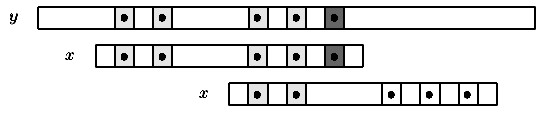
\includegraphics[width=4.25in, height=1in]{images/nohole}
        			\\ En este caso hay un mismatch en un \emph{no-hole}. En esta situación, no es necesario comparar los dos primeros
			    \emph{no-hole} del patrón luego del desplazamiento
		    \end{center}
        		\begin{itemize}
        			\item Si hay un mismatch en la segunda fase, entonces hay un sufijo del patrón que es igual a un factor del texto
        			y luego de desplazar correctamente estos seguirán coincidiendo y no es necesario volver a compararlos.
			\end{itemize}
			\begin{center}
        			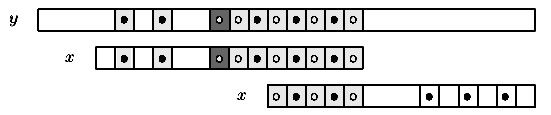
\includegraphics[width=4.25in, height=1in]{images/hole}
				\\En este caso, luego del shift, no hace falta comparar el prefijo que coincidió.
		    \end{center}
		\subsection{Implementación}
			Para la implementación de este algoritmo, se utiliza una serie de \emph{tablas} (implementadas como listas) para el
			preprocesamiento del patrón a buscar. Dichas tablas permiten realizar desplazamientos en el texto durante la comparación
			asegurándonos que no nos perderemos de nada y asegurándonos una mayor performance. \\
			\tab Dichas tablas son: \\ \\
			\tab\tab Kmin[$i$] = $\left\{ 
					\begin{array}{lcc}
             			d &   sii  & x[0 ... i - d - 1] = x[d ... i - 1] \wedge x[i - d] = x[i] \\
             			\\ 0 & sino
    					\end{array}
 		 		  \right.$
 		 	\\ \tab Esta tabla indica el shift que se debe realizar en caso de que la posición $i$ pertenezca a un \emph{no-hole}. \\
 		 	\tab\tab Rmin[$i$] = es el equivalente a Kmin pero para los \emph{hole}. \\
 		 	\tab Sea $ND + 1$ la cantidad de \emph{no-holes} en el patrón x, la tabla $h$ contiene a todos los \emph{no-holes} de
 		 	menor a mayor y luego a los $m - ND - 1$ \emph{holes} en orden decreciente. Esto es para recorrer a los \emph{no-holes}
 		 	de izquierda a derecha y a los \emph{holes} de derecha a izquierda. \\ \\
 		 	\tab\tab h[$i$] = $\left\{ 
					\begin{array}{lcc}
             			h[i] < h[i+1] (no-hole) &   si  & i \in [0, ND)\\
             			\\ h[i] > h[i+1] (hole) & si & i \in [ND, m)
    					\end{array}
 		 		  \right.$
 		 	\\ \\ \tab\tab first[$u$] = $v$, con $v$ entero más pequeño tal que $u \leq h[v]$. 
 		 	\\\\ \tab Para calcular el valor de Kmin, utilizamos la tabla hmax:
 		 	\\ \tab\tab hmax[$i$] es tal que: $\left\{ 
					\begin{array}{lcc}
             			x[i ... hmax[i] - 1] = x[0 ... hmax[i] - i -1]\\
             			\\ x[hmax[i]] \neq x[hmax[i] - i]
    					\end{array}
 		 		  \right.$
 		 	\\\\ \tab Finalmente, utilizamos la tabla \\
 		 	\tab\tab nhd0[$i$] = cantidad de \emph{no-holes} hasta la posición $i$. \\ \\
 		 	\tab Con estas tablas, armamos las dos tablas que realmente utilizamos en el algoritmo: \emph{shift} y \emph{next}. El
 		 	valor de ambas depende de si la posición $i$ contiene a un \emph{hole} o un \emph{no-hole} y se definen como:
 		 	\\ \tab\tab shift[$i$] = $\left\{ 
					\begin{array}{lcc}
             			kmin[h[i]] & si & i \in [0, ND)\\
             			\\ rmin[h[i]] & si & i \in [0, ND)
    					\end{array}
 		 		  \right.$
 		 	\\ \tab\tab next[$i$] = $\left\{ 
					\begin{array}{lcc}
             			ndh0[h[i] - kmin[h[i]]] & si & i \in [0, ND)\\
             			\\ ndh0[m - rmin[h[i]]] & si & i \in [0, ND)
    					\end{array}
 		 		  \right.$
 		 	\\ \tab Por lo tanto, si la ventana está ubicada en $T[j ... j + m - 1]$, cuando hay un mismatch entre $P[h[r]]$ y 
 		 	$T[j + h[r]]$, la ventana debe ser desplazada en \emph{shift[$r$]} y las comparaciones iniciarán desde la posición
 		 	\emph{h[next[$r$]]} del patrón. \\
 		 	\tab Por último, devolveremos un match sólo en dos casos:
 		 	\begin{itemize}
 		 		\item Si $i = m$.Arrancamos de $i=0$ y llegamos al final sin errores.
        			\item Si $j + m - 1 = j + h[i]$. Este es el caso en el que la comparación no empieza desde el inicio de P gracias
                 a algún dato del preprocessing y h[i] = m-1, es decir, llegamos al final de las comparaciones.
 		 	\end{itemize}
		
		\subsection{Complejidad}
			La complejidad de este algoritmo es $O(n + m)$, siendo $O(m)$ la etapa de preprocesamiento y $O(n)$ la etapa de búsqueda.
			En el peor de los casos, realiza $\frac{3}{2}n$ comparaciones, con $n$ la cantidad de caracteres del \emph{Texto} y $m$
			la cantidad de caracteres del \emph{Patrón}.
		
		\subsection{Características del algoritmo y casos de prueba}
			Este algoritmo tiene una característica importante y es que no es necesario conocer el alfabeto para buscar matches, pues
			en ningún momento es necesario conocer al mismo para ninguna de las tareas que se realizan en el mismo. \\
			\tab Es importante destacar que, si bien fue concebido como una mejora de KMP, en la mayoría de las pruebas que realizamos
			comparando el algoritmo ingenuo, MP, KMP y Colussi, este último fue el de peor performance. En el único caso en el que
			logramos que Colussi fuera el mejor fue un caso en el que teníamos un texto de la forma: \\
			\begin{verbatim}
			aaaaaaaaaaa#aaaaaaaaaaaaaa#aaaaaaaaaaa#....
			123456789#123456789#123456789#123456789#.....
			aaa..
			123..
			\end{verbatim}		
			\tab Con un patrón de la forma:
			\begin{verbatim}
			aaaaaaa#aaaaaa
			\end{verbatim}
			\tab En este caso, Colussi fue mucho mejor que los otros algoritmos previamente mencionados (aproximadamente un $50\%$ 
			mejor). Pero en todo el resto (archivos de ADN, textos en español, textos en inglés, código en C) tanto con texto largo
			y patrón corto como con texto corto y patrón largo, encontramos que este algoritmo no tuvo la performance esperada, siendo
			superado incluso por el algoritmo ingenuo.
			
	\section{Conclusiones generales}
		Luego del análisis de las pruebas para cada uno de los algoritmos analizados, sacamos las siguientes conclusiones:
		\begin{itemize}
			\item El algoritmo de Rabin-Karp alcanza su mayor performance cuando se realiza \emph{multiple string matching}.
			\item El algoritmo de Zhu-Takaoka es muy efectivo si se utiliza un alfabeto pequeño pero su performance se ve muy
			afectada cuando el alfabeto es grande, pues la etapa de preprocesamiento se hace muy larga.
			\item El algoritmo de Colussi, aunque es una optimización de KMP, en la mayoría de los casos no logra ser más veloz que
			KMP ni MP.
			\item En caso de no conocer la longitud del alfabeto o cómo está compuesto el mismo, es conveniente usar Colussi (o KMP).
			\item En caso de querer resolver el \emph{multiple string matching problem}, es conveniente utilizar el algoritmo de
			Rabin-Karp.
			\item En el caso de tener un alfabeto pequeño, el mejor algoritmo es el de Zhu-Takaoka.
			\item En el caso de tener un alfabeto grande, el mejor algoritmo es el de Colussi.
			\item Para el tamaño del texto, se respeta lo mencionado en los dos items previos; depende del tamaño del alfabeto.
			
		\end{itemize}
		
\end{document}
